
\newpage

\section{Разработка структуры приложения}

На данном этапе работы необходимо в соответствие с требованиями,
поставленными в техническом задании, разработать структуру конструктора
и описать основные алгоритмы функционирования.

\subsection{Разработка общей структуры конструктора }

Общая структура конструктора представлена на рисунке~\ref{f:general-struct}.

\begin{figure}[ht]
	\centering
	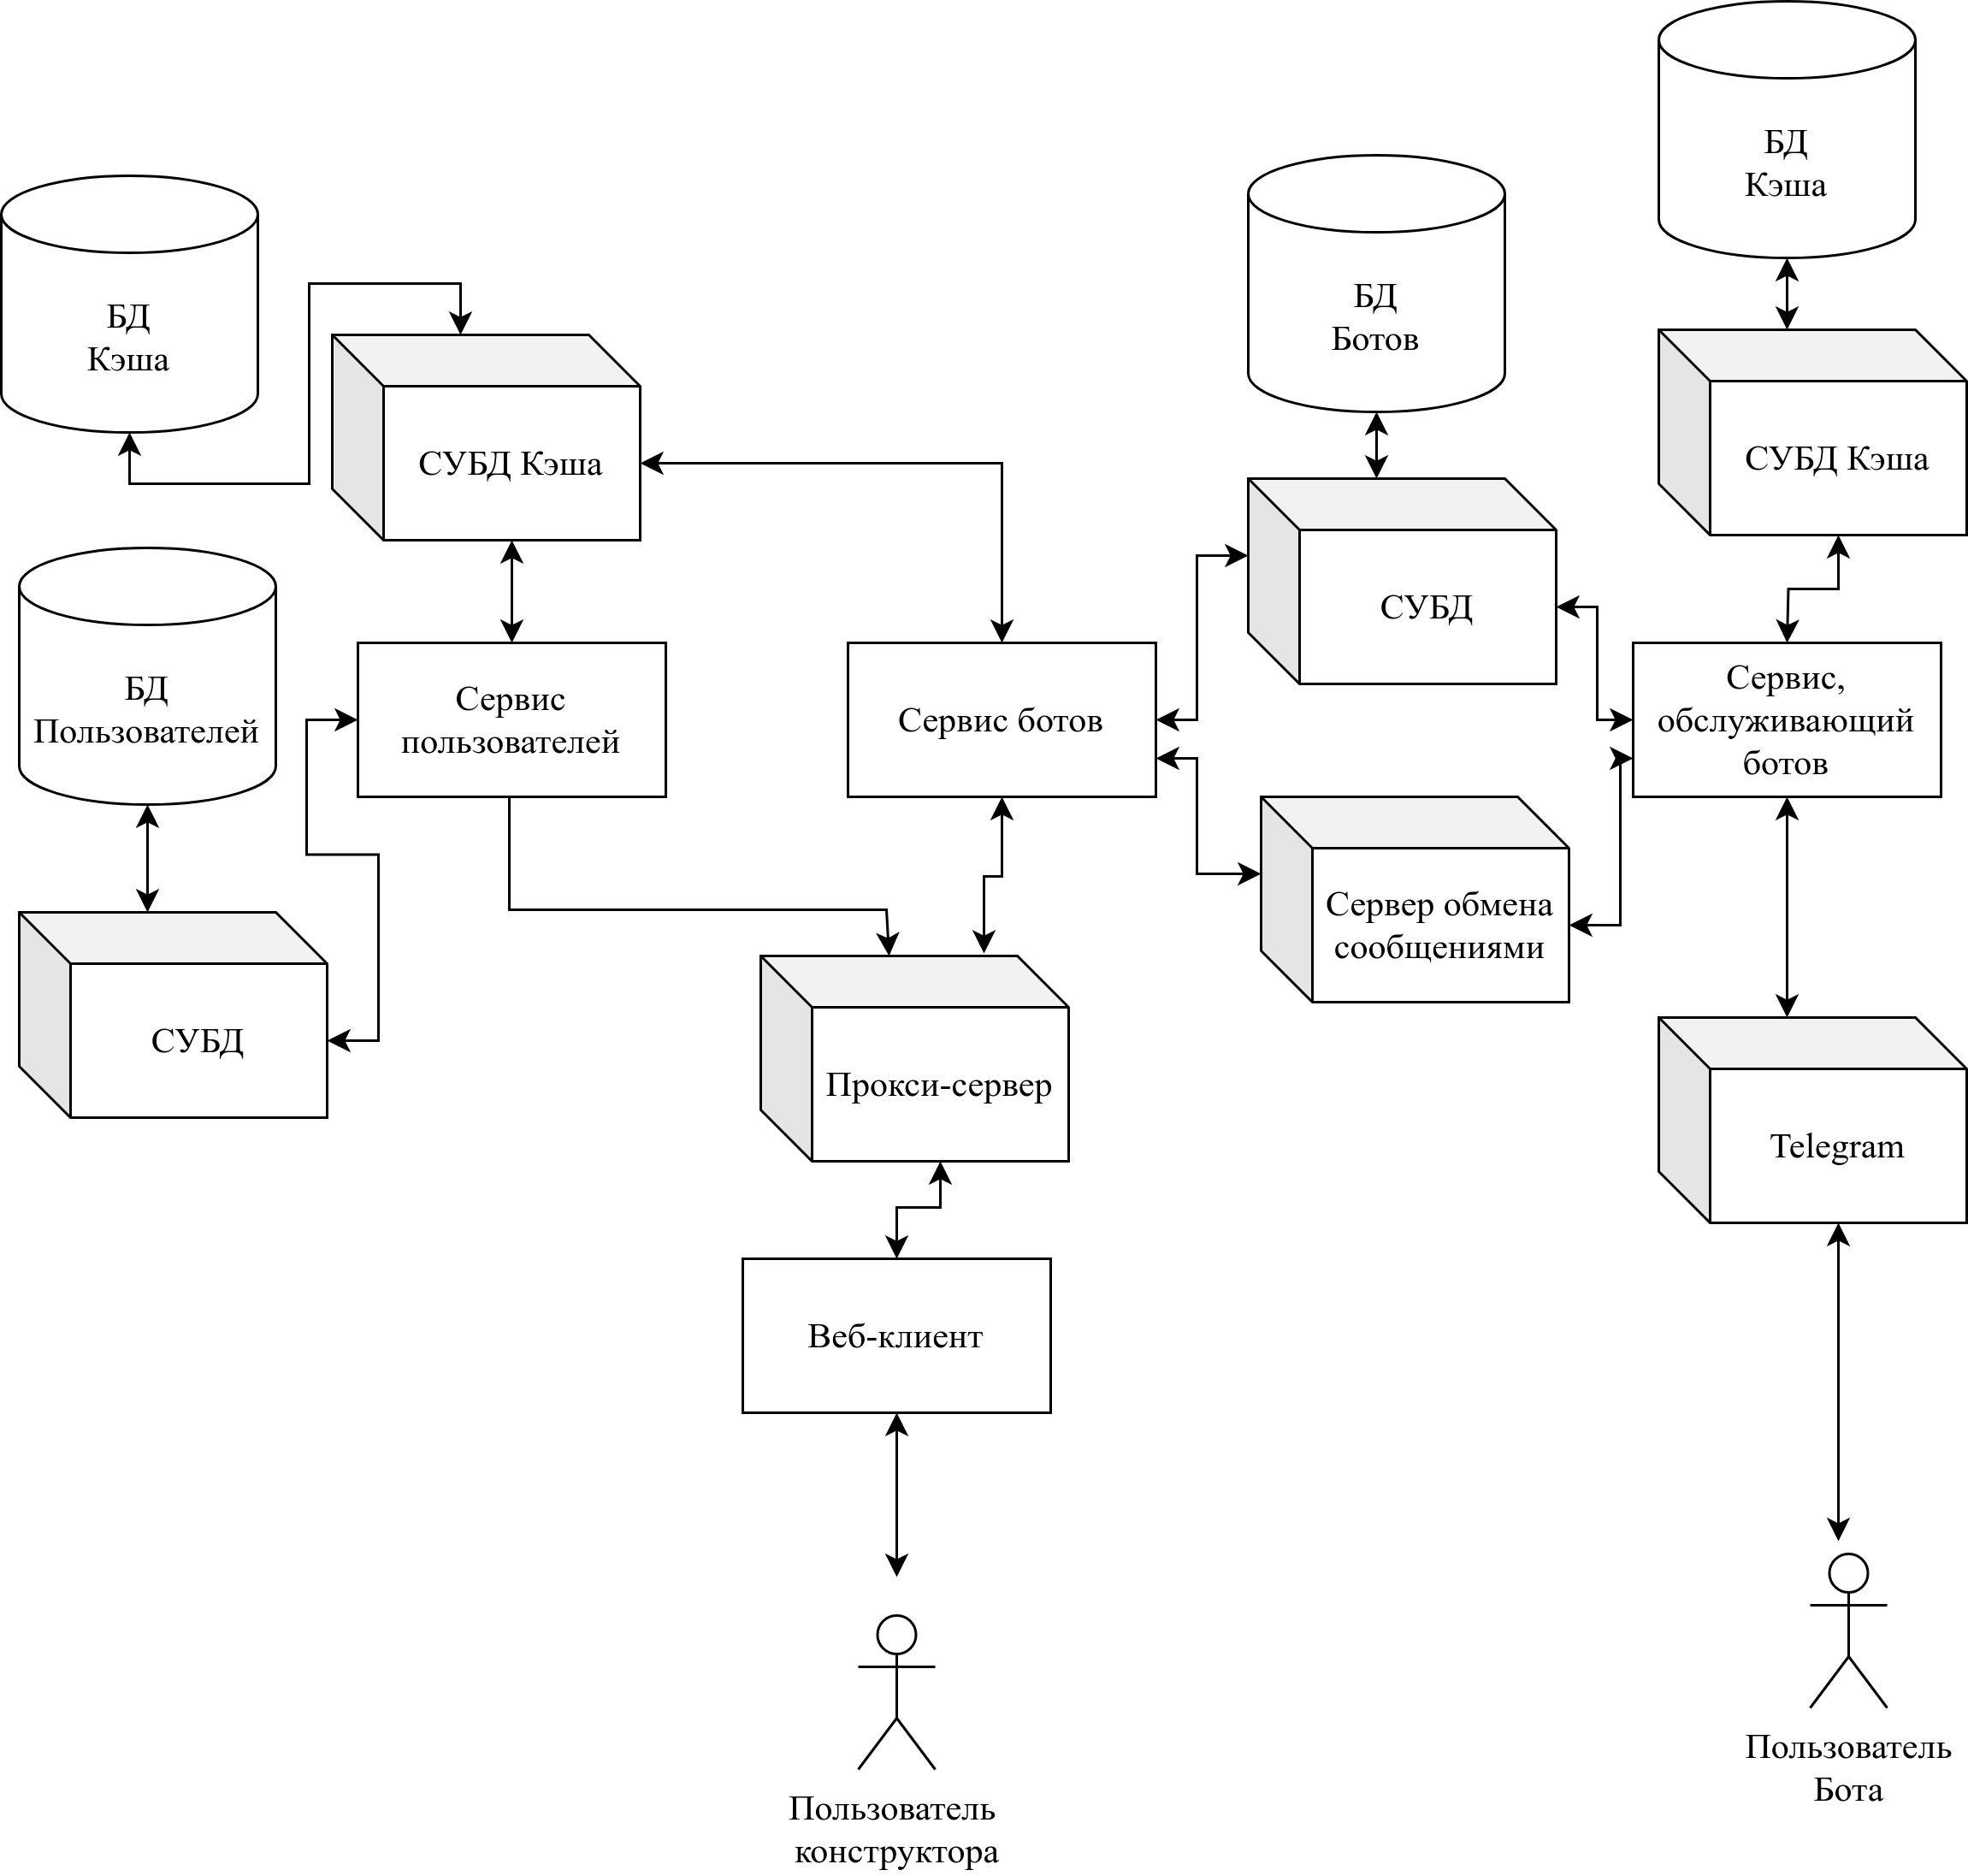
\includegraphics[width=0.95\textwidth]{structures/general}
	\caption{Общая структура конструктора}
	\label{f:general-struct}
\end{figure}


Конструктор состоит из серверной и клиентской части.

Серверная часть состоит из нескольких сервисов:
\begin{itemize}
	\item сервис пользователей;
	\item сервис ботов;
	\item сервис, обслуживающий ботов.
\end{itemize}

Сервис пользователей взаимодействует с хранилищами в виде базы
данных и кэша, в которых хранятся пользователи конструктора и их токены
авторизации. Через него происходит регистрация и аутентификация
пользователей.

Сервис ботов предоставляет программный интерфейс для работы с
ботами. Данный сервис выполняет следующие функции:
\begin{itemize}
	\item создание ботов;
	\item редактирование ботов;
	\item удаление ботов;
	\item запуск и остановка ботов.
\end{itemize}

Данные ботов сохраняются в базе данных. Авторизация пользователя
происходит с помощью данных из кэша пользователей.

Сервис, обслуживающий ботов, обрабатывает запросы от запущенных
Telegram ботов, также он получает и выполняет команды на запуск и
остановку ботов от сервиса ботов, команды при этом посылаются через сервер
обмена сообщениями. Данный сервис сохраняет и получает текущее состояние
пользователя из кэша.

Пользователь взаимодействует с конструктором через веб-интерфейс,
который через прокси-сервер связан с сервисами пользователей и ботов.
Веб-интерфейс является клиентской частью конструктора.


\subsection{Разработка структуры серверной части конструктора}


В данном разделе описываются разработанные структуры серверной части
конструктора и его основные алгоритмы функционирования.

\subsubsection{Модульная структура серверной части конструктора}

Модуль – набор структур и методов, который обобщает какую-то логику
приложения.

Модульная структура серверной части конструктора представлена на
рисунке~\ref{f:mod-server-struct}.

\begin{figure}[ht]
	\centering
	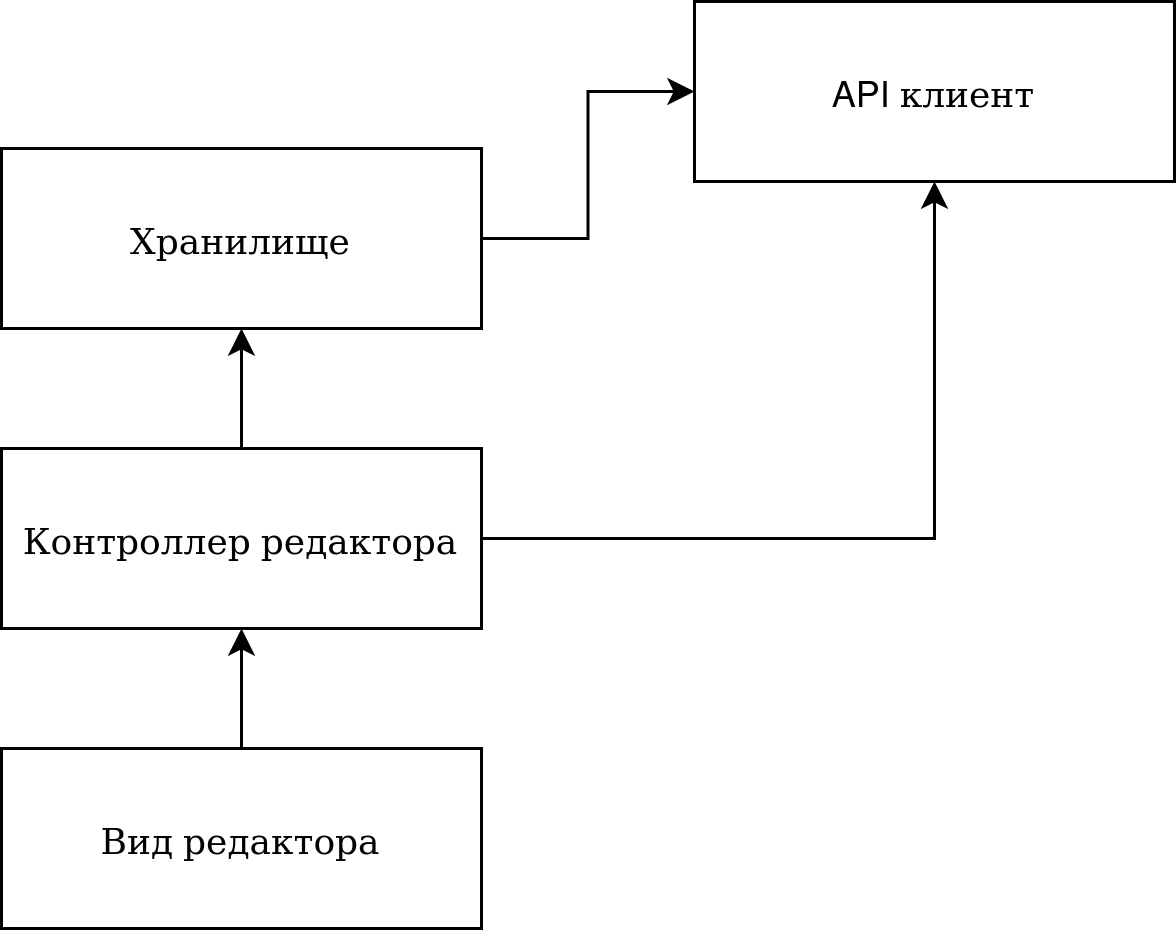
\includegraphics[width=0.8\textwidth]{structures/server/mod}
	\caption{Модульная структура серверной части конструктора}
	\label{f:mod-server-struct}
\end{figure}

Сервис ботов зависит от сервиса пользователей, который предоставляет
первому методы для авторизации пользователя. Также сервис ботов зависит
от модуля компонентов, который описывает структуры компонентов и
реализует их логику выполнения.

Для выполнения логики ботов сервис, обслуживающий ботов, вызывает
методы из модуля компонентов.

\subsubsection{Структура модуля компонентов}

Модуль компонентов состоит из следующих подмодулей:
\begin{itemize}
	\item подмодуль компонентов;
	\item подмодуль контекста;
	\item подмодуль исполнителя;
	\item подмодуль ввода-вывода.
\end{itemize}

Структура модуля компонентов представлена на рисунке~\ref{f:mod-comp-struct}.

\begin{figure}[ht]
	\centering
	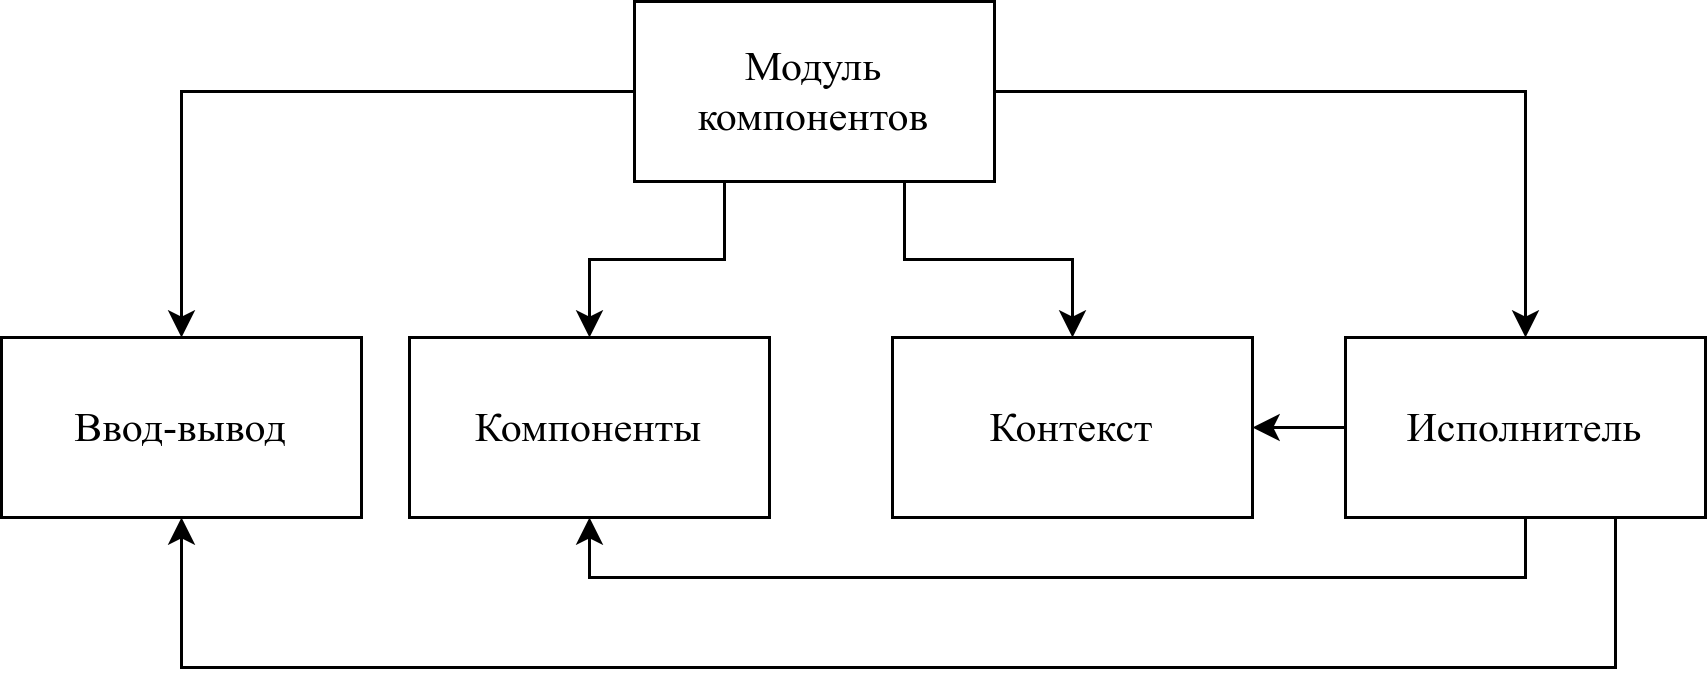
\includegraphics[width=0.8\textwidth]{structures/server/mod-comp}
	\caption{Структура модуля компонентов}
	\label{f:mod-comp-struct}
\end{figure}

Подмодуль компонентов содержит структуру и реализацию логики
компонентов. Каждый компонент реализует общий интерфейс компонента,
который определен в данном подмодуле.

В данном подмодуле определены следующие компоненты:
\begin{itemize}
	\item 	компонент ввода текста;
	\item 	компонент отправки сообщения;
	\item 	компонент вывода кнопок;
	\item 	компонент форматирования;
	\item 	компонент точки входа;
	\item 	компонент условия.
\end{itemize}

Подмодуль ввода-вывода предоставляет интерфейс, через который
окружение обменивается данными с рядом компонентов.

Подмодуль контекста содержит методы для работы с контекстом.
Контекст в рамках бота – память, с которой работают компоненты:
компоненты получают из контекста данные для выполнения и записывают в
него результат.

Исполнитель представляет собой объект, который содержит в себе
контекст и интерфейс ввода-вывода. Через него происходит выполнение
компонентов.


\subsubsection{Алгоритмы функционирования серверной части конструктора}

Пользователь конструктора взаимодействует с сервисом ботом, который
контролирует изменение данных и состояние ботов.
Схема алгоритма обработки запросов от пользователей сервиса ботов
представлен на рисунке~\ref{f:bot-service-alg}.

\begin{figure}[hp]
	\centering
	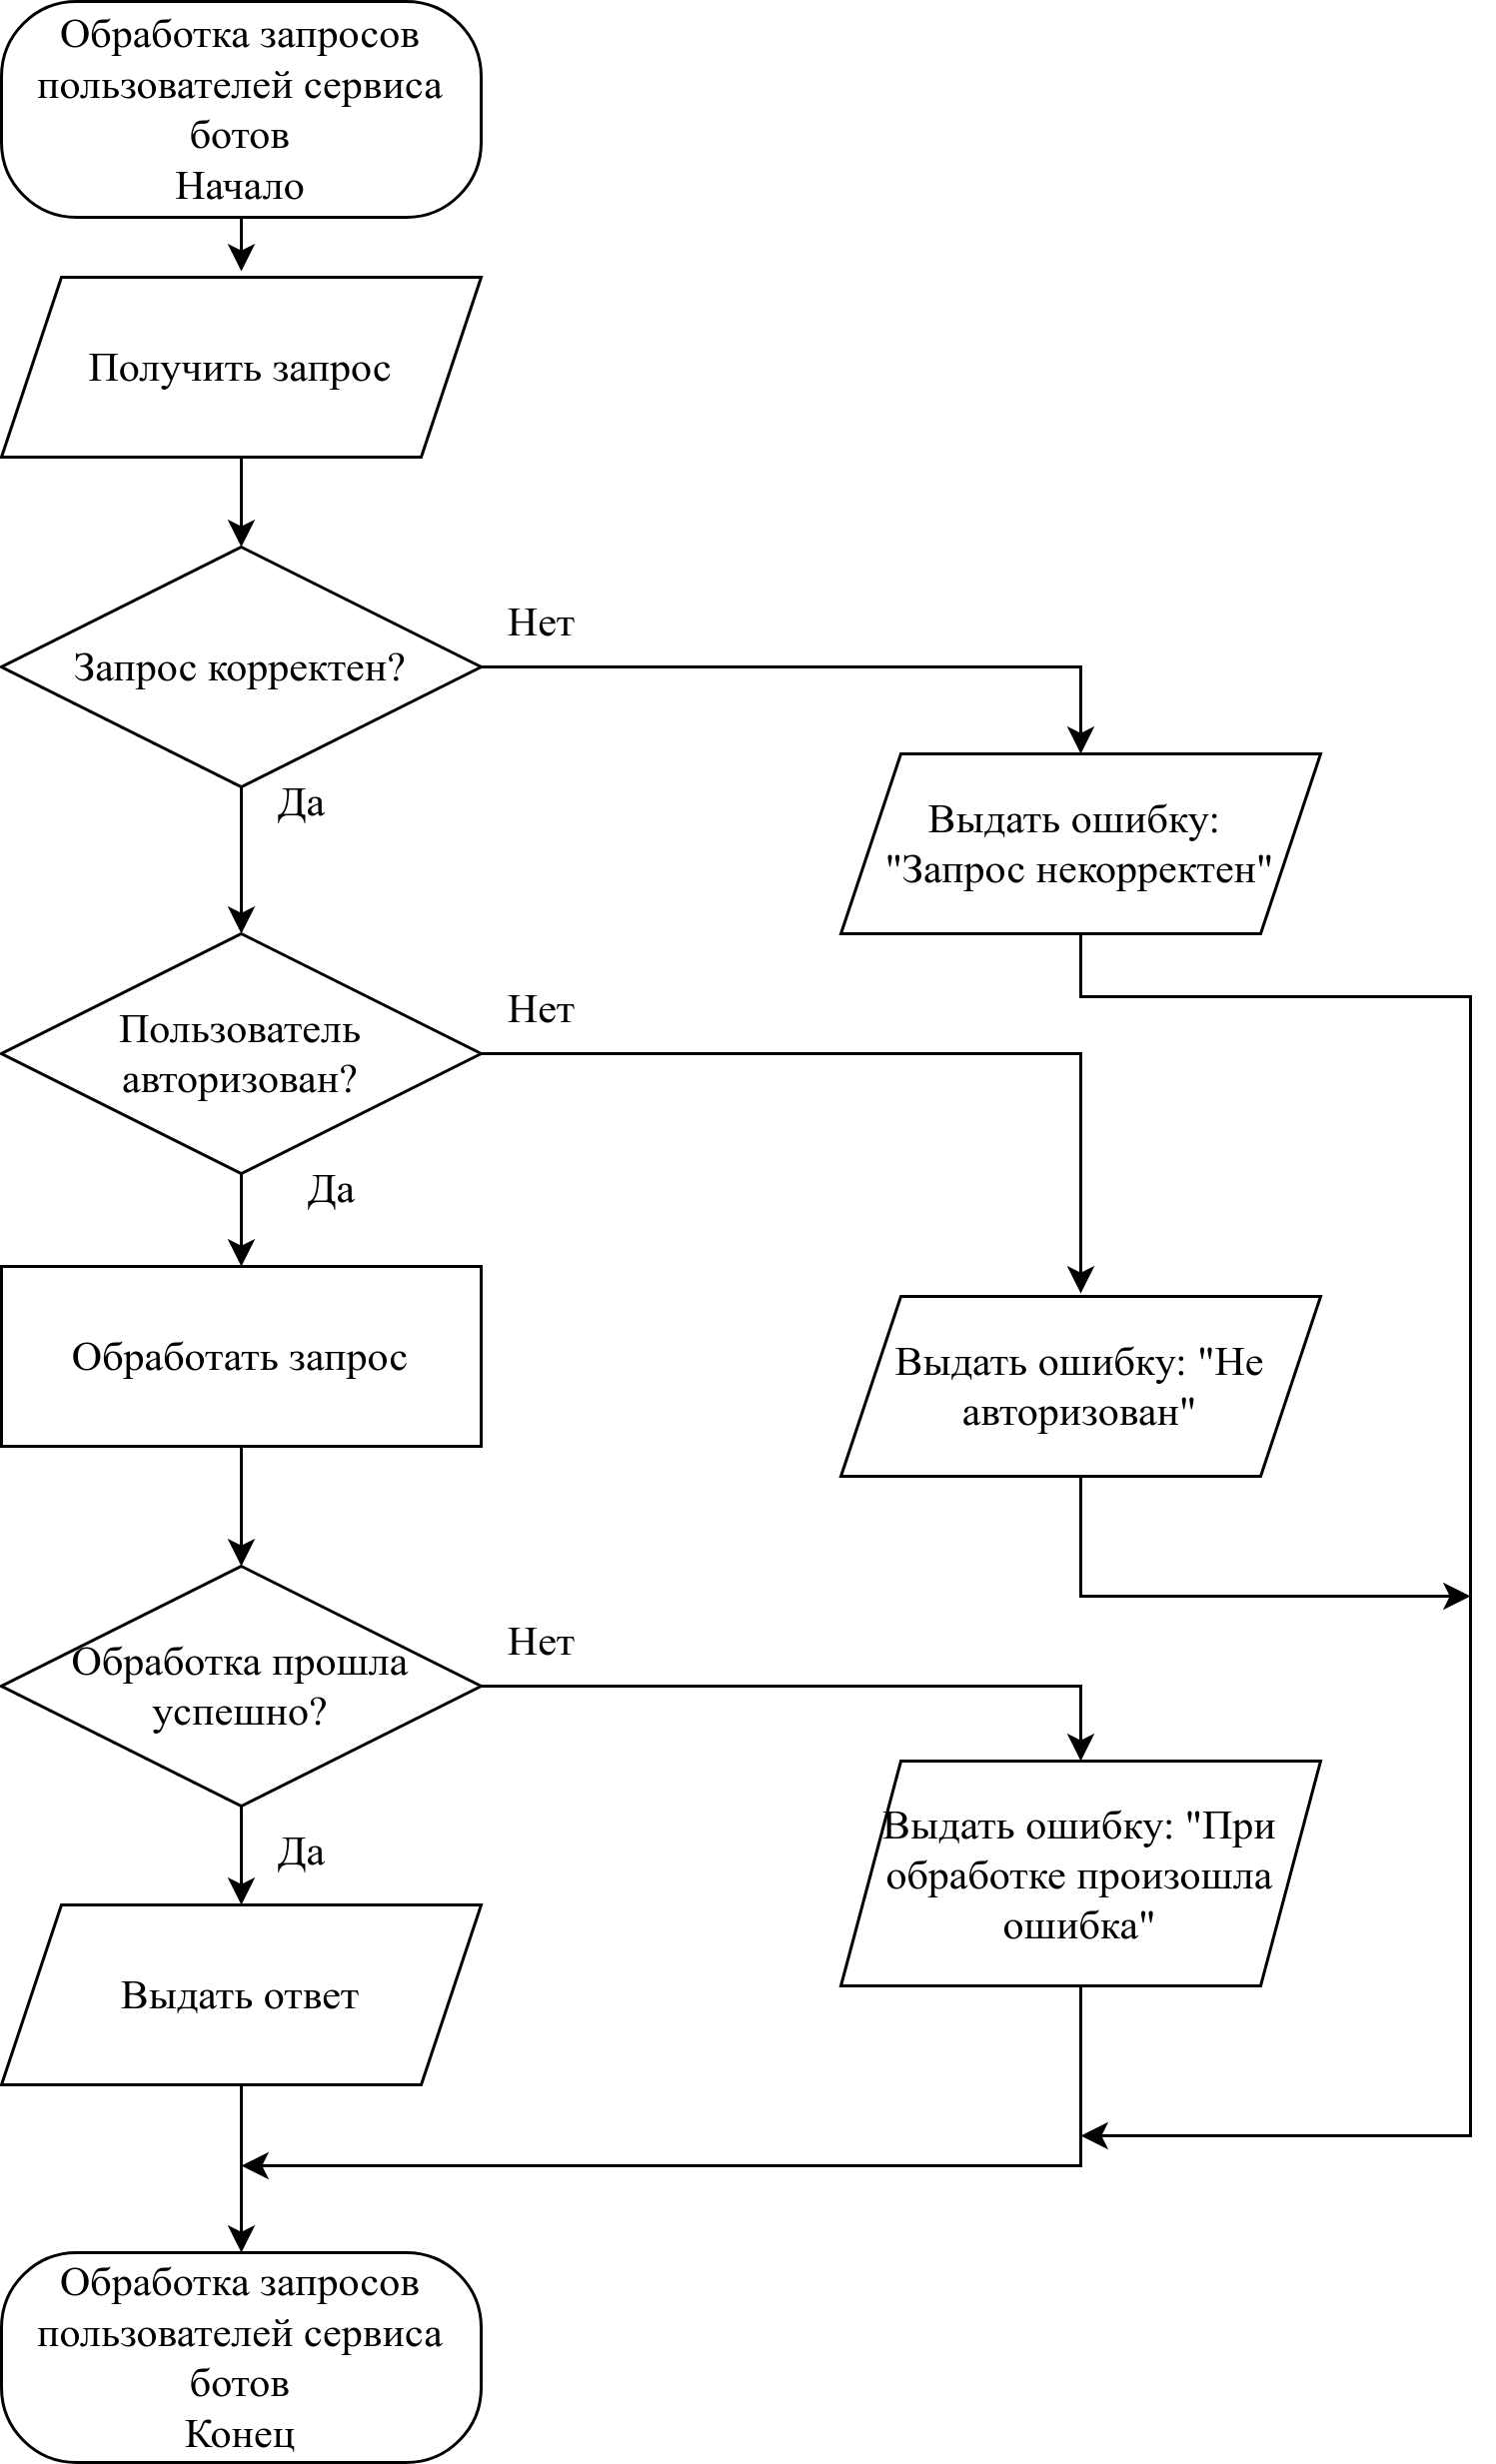
\includegraphics[height=0.9\textheight]{bot-service-alg}
	\caption{Схема алгоритма обработки запросов от пользователей сервиса ботов}
	\label{f:bot-service-alg}
\end{figure}

При получении запроса проверяется его корректность.
Если запрос не корректен, например, такое обращение не доступно, то
выводится соответствующая ошибка. Чтобы обработка прошла успешно, пользователь
должен быть авторизован в системе. В случае успешной обработки запроса выдается
ответ, иначе - ошибка.


При взаимодействии Telegram пользователя с ботом происходит
отправка запросов сервису, обслуживающему ботов, который в дальнейшем
обрабатывает данное событие. Схема алгоритма обработки запросов от
пользователя бота представлен на рисунке~\ref{f:bot-worker-alg}.


\begin{figure}[hp]
	\centering
	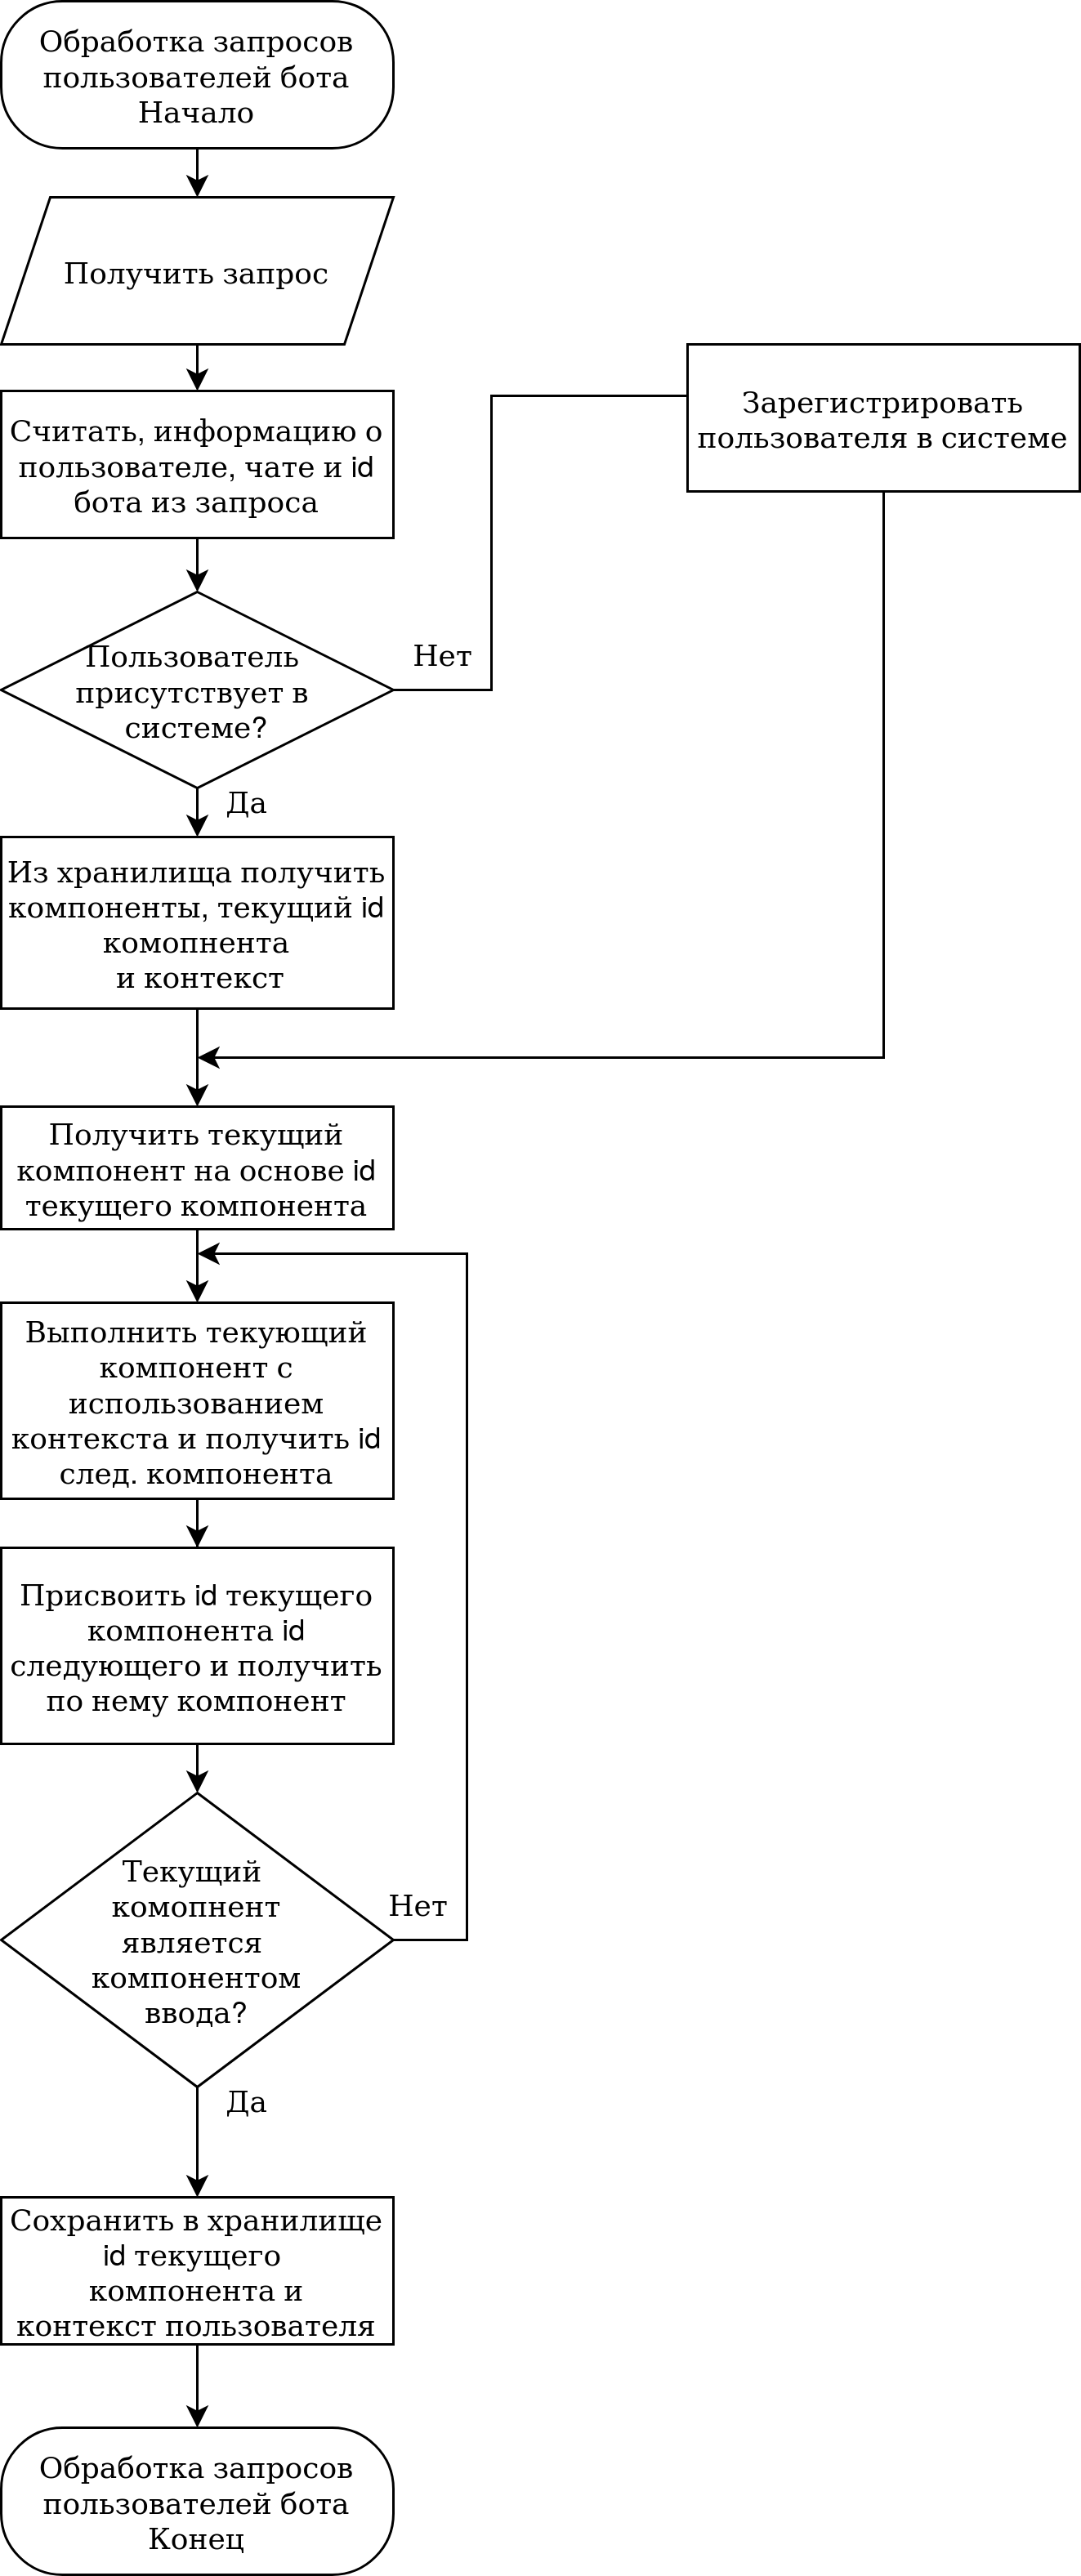
\includegraphics[height=0.9\textheight]{bot-worker-alg}
	\caption{Схема алгоритма обработки запросов от пользователей ботов}
	\label{f:bot-worker-alg}
\end{figure}

При принятии события сервисом происходит считывание следующих
данных:
\begin{itemize}
	\item информация о пользователе;
	\item информация о чате;
	\item id бота, от которого пришло сообщение.
\end{itemize}

На основе этих данных из хранилища идёт получение следующих
данных:
\begin{itemize}
	\item контекст пользователя;
	\item id текущего компонента пользователя;
	\item компонентов бота.
\end{itemize}

На основании id текущего компонента происходит получение текущего
компонента, который затем выполняется. Результат выполнения представляет
собой id следующего компонента, который присваивается текущему.

На основании следующего компонента принимается решение: если
компонент ожидает ввода каких-либо данных, то алгоритм заканчивается с
сохранением контекста и id текущего компонента, иначе идет выполнение
следующего компонента.

\newpage

\subsubsection{Обеспечение защиты информации клиентов конструктора}

\subsection{Разработка структуры клиентской части конструктора}


В данном разделе описываются разработанные структуры клиентской части
конструктора и его диаграммы состояний.

\subsubsection{Структура интерфейса конструктора}

Пользовательский интерфейс конструктора представляет собой
административную панель с набором следующих страниц:

\begin{itemize}
	\item страница аутентификации;
	\item страница регистрации;
	\item страница ботов пользователя конструктора;
	\item страница создания нового бота;
	\item страница запуска бота;
	\item страница редактирования бота.
\end{itemize}


Каждая страница состоит из верхней панели и содержимого страницы.
Верхняя панель содержит ссылки на страницы аутентификации и регистрации,
если пользователь не вошёл в систему, иначе - кнопку “выйти из системы”.

Страница аутентификации и регистрации содержат поля ввода логина и
пароля пользователя, под которым располагается кнопка входа или
регистрации. Шаблон содержимого страницы аутентификации представлен на
рисунке

\paragraph{Длинный длинный длиннный длинный длинный длиннный длинный длинный длинный текст}



